% !TEX root = slides.tex
%%%%%%%%%%%%%%%%%%%%%%%%%%%%%%%%%%%%%%%%%%%%%%%%%%%%%%%%%%%%

\begin{frame}[t]
\frametitle{Bayesian Framework for Model Error Estimation}

\medskip
\centerline{
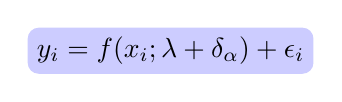
\begin{tikzpicture} \node [rounded corners,fill=blue!20] {
$y_i=f(x_i;\lambda+\delta_\alpha)+\epsilon_i$
};
\end{tikzpicture}
}

\bi
\item Given data $y_i$, perform \emph{simultaneous} estimation of $\tlam=(\lambda,\alpha)$,\\i.e. model parameters $\lambda$ and model-error parameters $\alpha$.
\item Bayes' theorem
\[
\overbrace{p(\tlam|y)}^{\textrm{Posterior}}= \frac{\overbrace{p(y|\tlam)}^{\textrm{Likelihood}} \overbrace{p(\tlam)}^{\textrm{Prior}}}{\underbrace{p(y)}_{\textrm{Evidence}}}
\]

\vspace*{2mm}

\item In order to estimate the likelihood $L_y(\tlam)=p(y|\tlam)=p(y|\lambda,\alpha)$, \\one needs uncertainty propagation through  $\;f(x_i;\underbrace{\lambda+\delta_\alpha}_{\textrm{stochastic}})$,
\vspace*{2mm}

\item ... hence, we employ Polynomial Chaos (PC) representation for $\delta_\alpha$.
\ei
\end{frame}